\documentclass[tikz,border=4pt]{standalone}
% Shared look for the per-pattern diagrams. Copied from the IATEFL LTSIG talk
% (talks/doubly-personalised-language-learning/figures/llm-patterns.tex).
\usepackage{amssymb}
\usepackage{fontspec}
\setmainfont{Helvetica Neue}
\usetikzlibrary{arrows.meta,positioning,calc,fit}
\definecolor{ink}{HTML}{23373B}
\definecolor{hlc}{HTML}{C2410C}
\definecolor{okc}{HTML}{2E7D32}
\definecolor{badc}{HTML}{B91C1C}
\tikzset{
  mini/.style={rounded corners=2pt, minimum height=7mm, align=center,
               font=\small\color{ink}, fill=white, draw=ink!70, line width=0.6pt, inner sep=3pt},
  minillm/.style={mini, fill=hlc, draw=hlc, font=\small\bfseries\color{white}},
  fixed/.style={mini, fill=ink!12},                 % the fixed part of a prompt
  sarr/.style={-{Stealth[length=2mm]}, ink, line width=0.8pt},
  lbl/.style={font=\footnotesize\itshape\color{ink!75}},
  ok/.style={font=\small\bfseries\color{okc}},
  bad/.style={font=\small\bfseries\color{badc}},
}

% LLM Content Validation Tracking: every stored LLM-generated record carries a
% trust level. Events raise it (above); each consumer reads only the levels it
% can tolerate (brackets below). A state, not a flow, so no arrows.
\begin{document}
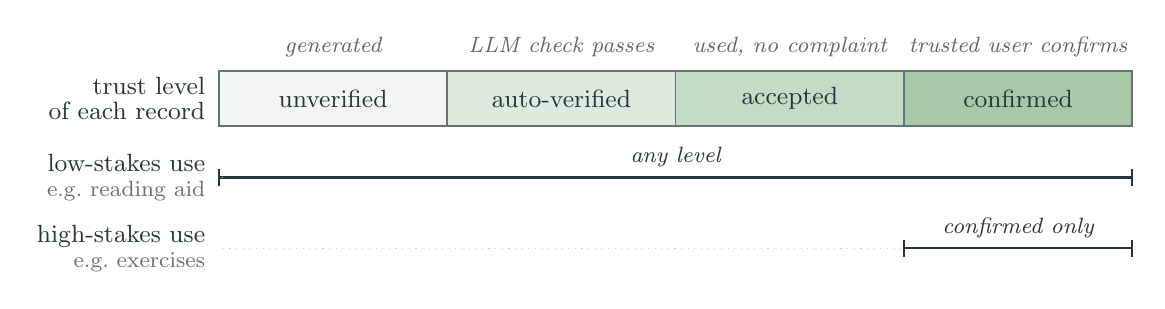
\begin{tikzpicture}[
  lvl/.style={mini, rounded corners=0pt, minimum width=29mm, inner sep=2pt},
  ev/.style={lbl, anchor=south, yshift=0.5mm},
  span/.style={ink, line width=0.8pt, |-|},
  use/.style={font=\small\color{ink}, anchor=east, align=right}]
\node[lvl, fill=okc!6]  (a) at (0,0)   {unverified};
\node[lvl, fill=okc!16] (b) at (2.9,0) {auto-verified};
\node[lvl, fill=okc!28] (c) at (5.8,0) {accepted};
\node[lvl, fill=okc!42] (d) at (8.7,0) {confirmed};
\node[ev] at (a.north) {generated};
\node[ev] at (b.north) {LLM check passes};
\node[ev] at (c.north) {used, no complaint};
\node[ev] at (d.north) {trusted user confirms};
\node[use, anchor=east] at (-1.5,0) {trust level\\[-2pt]of each record};

\draw[span] (a.west |- 0,-1.0) -- node[above, lbl] {any level} (d.east |- 0,-1.0);
\node[use] at (-1.5,-1.0) {low-stakes use\\[-2pt]{\footnotesize\color{ink!70} e.g.\ reading aid}};
\draw[span] (d.west |- 0,-1.9) -- node[above, lbl] {confirmed only} (d.east |- 0,-1.9);
\node[use] at (-1.5,-1.9) {high-stakes use\\[-2pt]{\footnotesize\color{ink!70} e.g.\ exercises}};
\draw[ink!25, dotted] (-1.4,-1.9) -- (d.west |- 0,-1.9);
\draw[ink!25, dotted] (-1.4,-1.0) -- (a.west |- 0,-1.0);
\end{tikzpicture}
\end{document}
